% !TEX root = Projektdokumentation.tex


\section{Datenbankänderung}

\subsection{Bestehende Datenbank}

Für die Behebung der bestehenden Fehlern sowie für die Erstellung neuer Funktionalitäten war es wichtig, einen exakten Überblick über die Datenbank zu besitzen. Da zu Beginn nur eine veraltete Übersicht über die Tabellen vorhanden waren, musste diese zuerst aktualisiert werden. Die erstellte Übersicht ist im Anhang unter \glqq Datenbank aktueller Zustand \grqq auf Seite \hyperlink{page.\getpagerefnumber{pdf:dbVorVeraenderung}}{\getpagerefnumber{pdf:dbVorVeraenderung}} zu finden.



\subsection{Änderung an der Datenbank}
\label{subsec:DBAenderungen}
Verschiedene neue Funktionalitäten verlangten eine Änderung der Datenbank, da neue Arten von Daten abgespeichert werden mussten.


\begin{figure}
	\centering
	\begin{subfigure}{.5\textwidth}
		\centering
		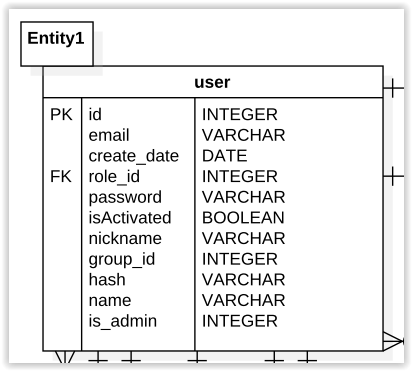
\includegraphics[width=0.6\textwidth]{Images/DB_User_Table.PNG}
		\caption{Alte User-Tabelle}
	\end{subfigure}%
	\begin{subfigure}{.5\textwidth}
		\centering
		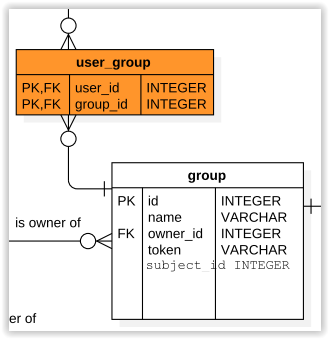
\includegraphics[width=0.6\textwidth]{Images/DB_Group_Table.PNG}
		\caption{Alte User-Tabelle}
	\end{subfigure}
\end{figure}



\begin{itemize}
	\item Gruppenmanagement\\
	Ein Benutzer konnte bisher nur einer Gruppe zugeordnet sein. Wie auf dem Bild a) ersichtlich, war deren ID direkt in der Tabelle \glqq User\grqq gespeichert. Neu sollte eine Gruppe mehrere Benutzer beinhalten und ein Benutzer in mehreren Gruppen sein können. Es wurde deshalb, wie auf Bild b) ersichtlich, eine Zwischentabelle für die Auflösung der N:M - Beziehung gemacht.\\
	Mehrere Gruppen werden unter anderem dafür benötigt, dass ein Benutzer neu seine Themenbereich-Interessen angeben kann und dafür je einer Gruppe zugeordnet ist. Dabei soll er auch weiterhin Praktikums- oder Vorlesungsgruppen zugeordnet sein.
	\item Quiz-Durchführungen\\
	Da es im Modul \gls{CN1} mehrere Praktikumsgruppen gibt, welche unterschiedliche Zeiträume für die Lösung von Quizzes zur Verfügung haben, benötigte es pro Quiz mehrere Durchführungen. Dies führte ebenfalls Änderungen an der Datenbank. \\
	Neu können mehrere Durchführungen erstellt und zu diesen Gruppen zugeordnet werden. So kann ein Enddatum pro Gruppe festgelegt werden.
	Dafür mussten in der Datenbank einige Änderungen vorgenommen werden. 
	
	Die Wichtigste dieser Änderungen war das Erstellen der execution Tabelle. Die bisherigen Einstellungen für eine Durchführung eines Quizzes wurden aus der Tabelle questionnaire in die Tabelle execution übertragen.
	
	Es wurden mehrere Verknüpfungstabellen nötig, welche dafür sorgen, dass Quizzes, Teilnehmer und Gruppen einer Durchführung zugeordnet werden können.
	
	Schlussendlich wurde die Tabelle priority\_settings erstellt. In dieser werden vom Standard abweichende Einstellungen eines Erstellers abgespeichert. Bei der Erstellung einer neuen Durchführung werden dann diese Werte als Startwerte eingetragen anstatt der Standardwerte. Das Ziel dahinter ist, dass der Ersteller so wenig wie möglich von Hand einstellen muss, sobald er seinen Durchführungstyp beziehungsweise seine Durchführungspriorität (Lernhilfe, Testatbedingung, Prüfung) gewählt hat.
	
	In der untenstehenden Grafik sind alle Datenbankänderungen festgehalten, dabei sind die neu erstellten Tabellen orange ausgefüllt und die veränderten Tabellen orange umrahmt.
	
	\begin{figure}[H]
		\centering
		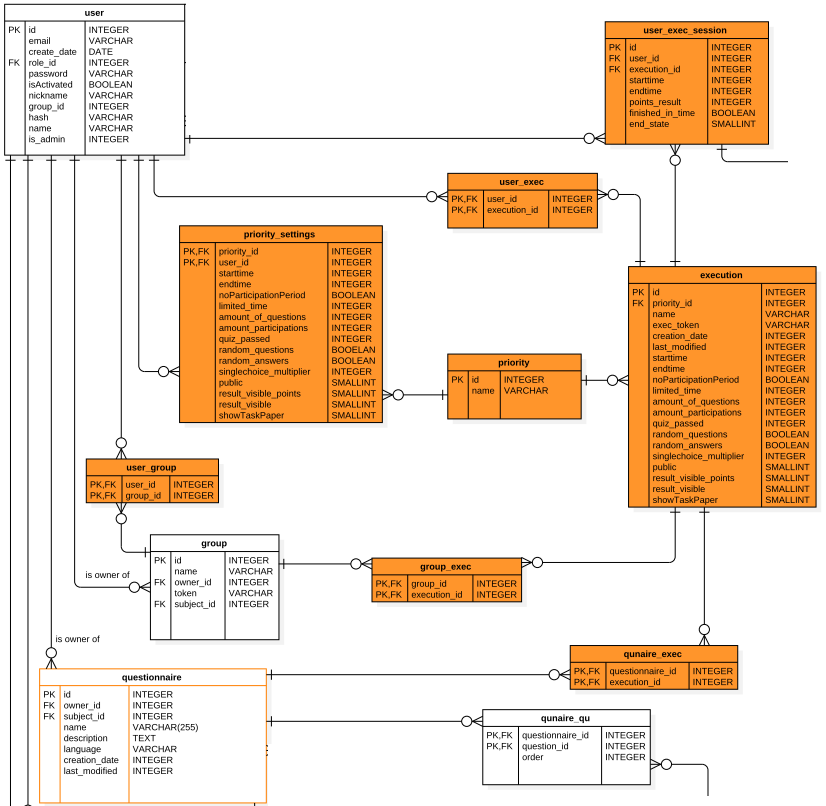
\includegraphics[width=1\textwidth
		]{Images/DB_Execution_Table.PNG}
		\caption{Datenbankänderungen für die Durchführung}
	\end{figure}
	
\end{itemize}

Diese umfangreichen Datenbank-Änderungen zogen viele Anpassungen der Datenbankabfragen nach sich, da beim bisherigen questionnaire viele Verbindungen zusammenliefen. So musste von der Quiz-Erstellung, über die Quiz-Durchführung bis zur PDF-Generierung der Auswertung vieles umgeschrieben werden.
